%! TeX program = lualatex
\documentclass[main]{subfiles}

\begin{document}

\title[AutoML: HPO]{Grid Search and Random Search}
\subtitle{The Bad and the Ugly}
\author[Lars Kotthoff]{Lars Kotthoff}
\date{}

\titlebackground*{images/AutoML_HPO_2_2}

%\institute{}
%\date{}
	
	\maketitle
	

\begin{frame}{Grid Search}
    \begin{columns}
        \column{.5\textwidth}
        \begin{itemize}
            \item Discretize all hyperparameters along a grid, then try all values
            \item Easy to implement and easily parallelizable
            \item Scales exponentially in the number of hyperparameters (curse of dimensionality), searches irrelevant areas
            \item Discretization can be arbitrary and is not straightforward
        \end{itemize}

        \column{.5\textwidth}
        \begin{center}
            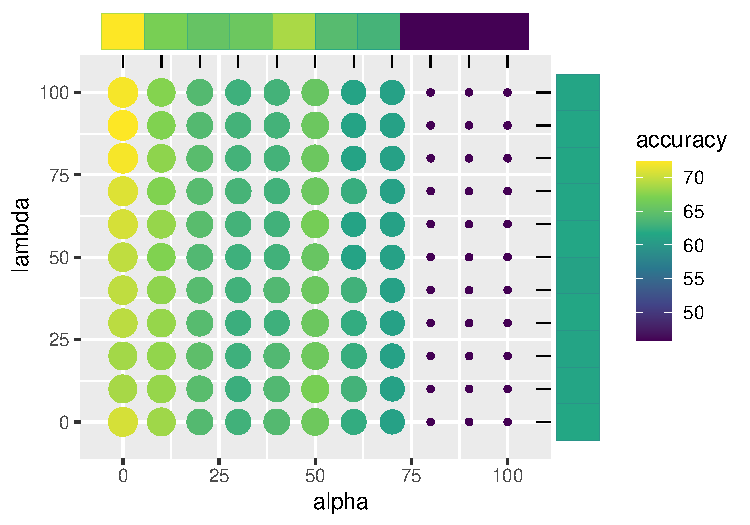
\includegraphics[width=\textwidth]{images/grid}
        \end{center}
    \end{columns}
\end{frame}

%----------------------------------------------------------------------

\begin{frame}{Random Search}
    \begin{columns}
        \column{.5\textwidth}
        \begin{itemize}
            \item Uniformly sample from the configuration space
            \item Also easy to implement and easily parallelizable
            \item Can control easily how much to sample
            \item Also searches irrelevant areas, but better coverage of the space than grid search, in particular if some dimensions are unimportant~\liturl{Bergstra and Bengio 2012}{https://www.jmlr.org/papers/volume13/bergstra12a/bergstra12a.pdf}
            \item Often performs better than grid search in practice
        \end{itemize}

        \column{.5\textwidth}
        \begin{center}
            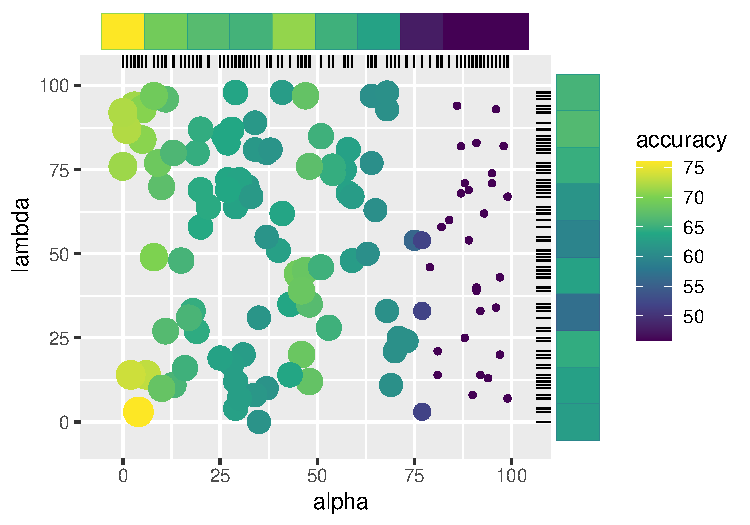
\includegraphics[width=\textwidth]{images/random}
        \end{center}
    \end{columns}
\end{frame}

%----------------------------------------------------------------------

\begin{frame}{Summary} 
\begin{enumerate}
    \item Grid search: try all possible values along a grid
    \item Random search: sample uniformly from the configuration space
    \item Random search often useful baseline or to gauge difficulty of HPO task
\end{enumerate}
\end{frame}

\end{document}
